\chapter{Конструкторская часть}

\section{Разработка алгоритмов}

На рисунке \ref{img:floyd} представлена схема последовательного алгоритма Флойда, на рисунке \ref{img:parallel} - параллельного. Схема алгоритма нахождения крайтчайшего расстояния между двумя вершинами показана на рисунке \ref{img:min}. Схема организации многопоточности представлена на рисунке \ref{img:threads}. Семафоры и мьютексы не используются.

\begin{figure}[H]
	\begin{center}
		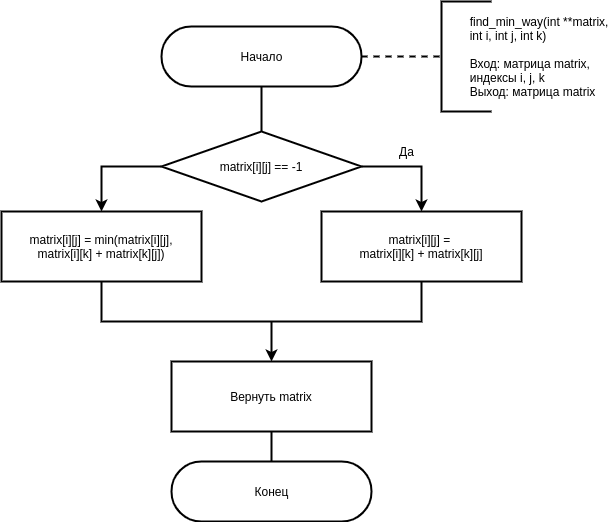
\includegraphics[scale=0.6]{images/min.png}
	\end{center}
	\captionsetup{justification=centering}
	\caption{Алгоритм нахождения кратчайшего пути между двумя вершинами}
	\label{img:min}
\end{figure}

\begin{figure}[H]
	\begin{center}
		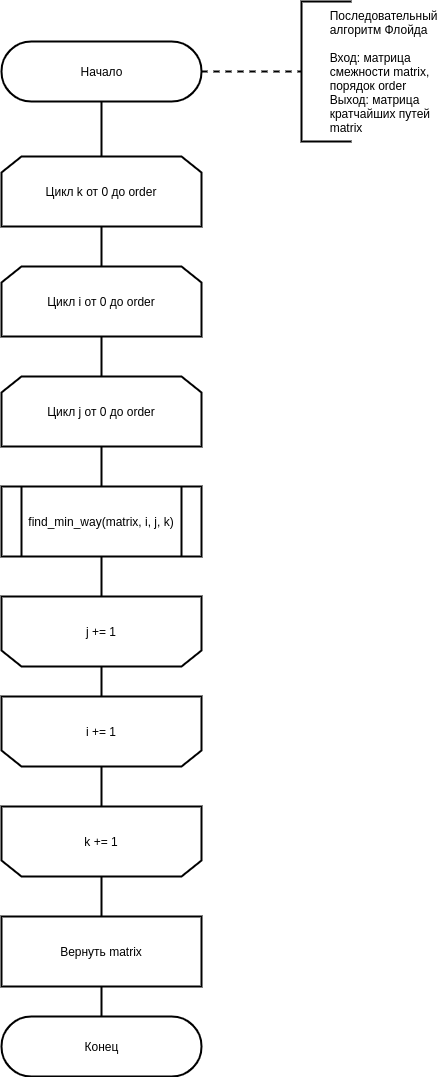
\includegraphics[scale=0.6]{images/floyd.png}
	\end{center}
	\captionsetup{justification=centering}
	\caption{Последовательный алгоритм Флойда}
	\label{img:floyd}
\end{figure}

\begin{figure}[H]
	\begin{center}
		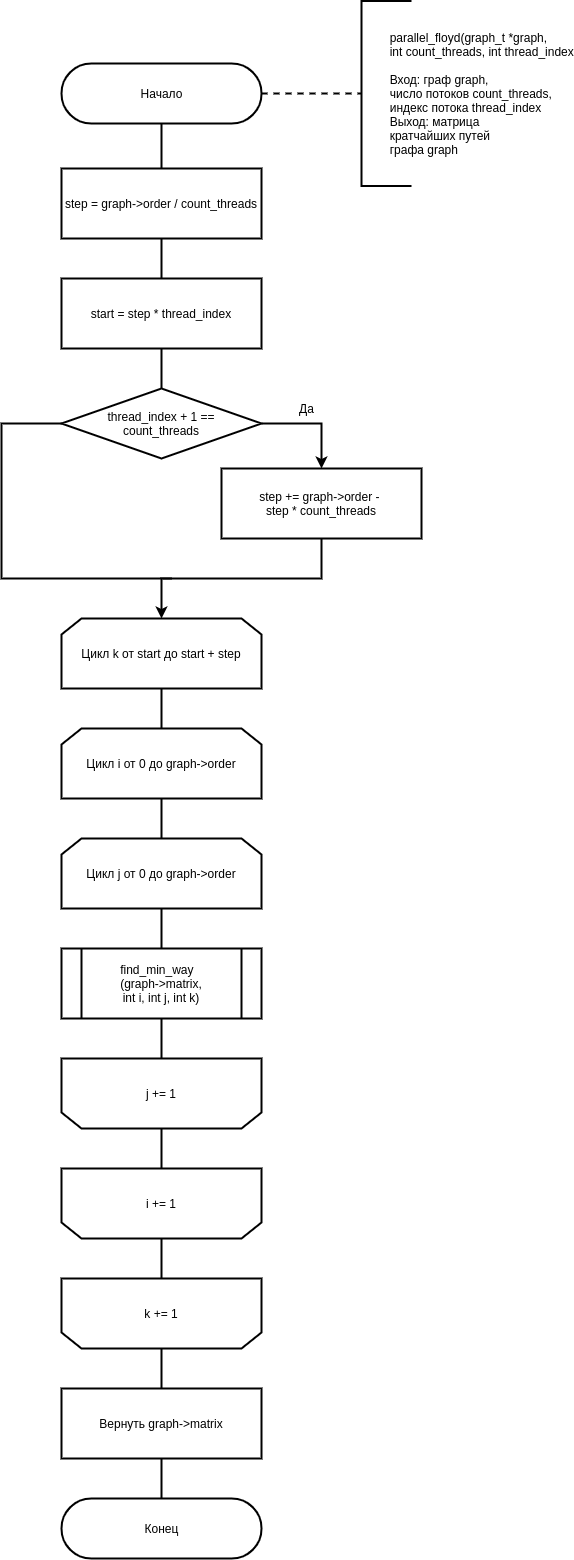
\includegraphics[scale=0.4]{images/parallel.png}
	\end{center}
	\captionsetup{justification=centering}
	\caption{Параллельный алгоритм Флойда}
	\label{img:parallel}
\end{figure}

\begin{figure}[H]
	\begin{center}
		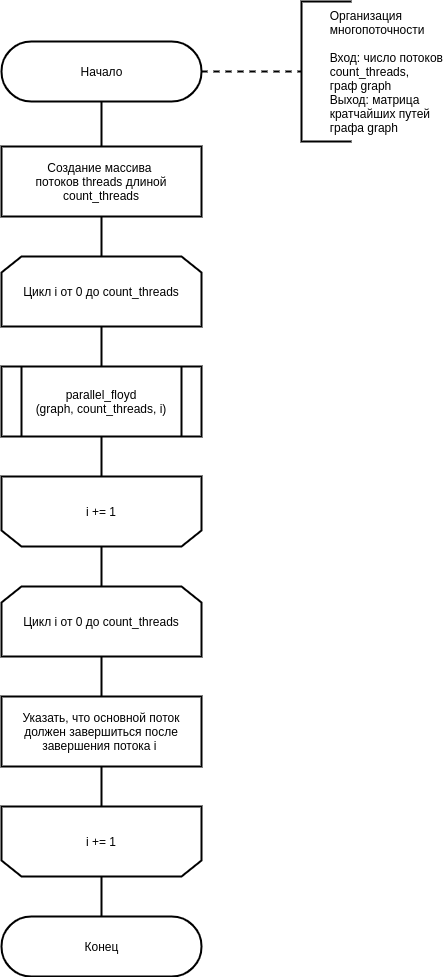
\includegraphics[scale=0.6]{images/threads.png}
	\end{center}
	\captionsetup{justification=centering}
	\caption{Организация многопоточности}
	\label{img:threads}
\end{figure}
